\documentclass[xcolor=pdftex,dvipsnames,table]{beamer}
\mode<presentation>
\usetheme{boxes}
\setbeamertemplate{navigation symbols}{}
% http://www.latex-community.org/forum/viewtopic.php?f=4&t=6694
\setbeamertemplate{navigation symbols}{\raisebox{5pt}{\makebox[\paperwidth]{\hfill\makebox[10pt]{\scriptsize\insertframenumber\vspace{1ex}}}}}
\setbeamertemplate{footline}[frame number]
\setbeamertemplate{blocks}[shadow=false]
\setbeamercolor*{block title}{fg=structure,bg=RoyalBlue!10}
\setbeamercolor*{block title example}{fg=BrickRed,bg=Goldenrod!10}
\setbeamercolor*{block title alerted}{fg=white,bg=black}
\addtobeamertemplate{block begin}{\pgfsetfillopacity{0.8}}{\pgfsetfillopacity{1}}
\rowcolors{1}{RoyalBlue!20}{RoyalBlue!5}

%\DeclareGraphicsRule{*}{mps}{*}{}

\usepackage{latexsym}
\usepackage{hyperref}

\raggedright

\newcount\lecturecount
\lecturecount=0
\AtBeginLecture{%
    \advance\lecturecount by 1
    \date{}
    \begin{frame}
    \begin{center}
    \titlepage
    \ifnum\lecturecount=1
    Part \the\lecturecount: \insertlecture
    \else
    Part \the\lecturecount: \insertlecture
    \fi
    \end{center}
    \end{frame}
}

\ifx\pdfoutput\undefined
%  \usepackage{graphicx}
\else
%  \usepackage[pdftex]{graphicx}
  \DeclareGraphicsRule{*}{mps}{*}{}
\fi
%\usepackage{cgloss4e,gb4e}
%\usepackage{qtree}
%\usepackage{tree-dvips}

\raggedright

\definecolor{bgblue}{rgb}{0.04,0.39,0.53}

\begin{document}

\title{\color{blue}Natural Language Processing}

\author{Anoop Sarkar \\ {\tt http://anoopsarkar.github.io/nlp-class}}
\institute{}
%\date{}
     
{
\setbeamertemplate{navigation symbols}{}
\addtocounter{framenumber}{-1}
\begin{frame}
\begin{center}
\vspace{1cm}
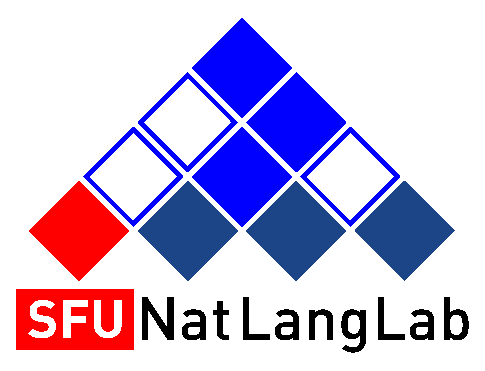
\includegraphics[scale=0.4]{figures/natlang-cky-logo.eps}
\end{center}
\titlepage
\end{frame}
}



\begin{frame}
\frametitle{Parts of Speech}
\begin{itemize}
\item We have seen that individual words can be classified into groups
  or classes that we call {\bf parts of speech}
\begin{itemize}
\item Determiners: {\em a, the}
\item Verbs: {\em arrive, attracts, love, sit}
\item Prepositions: {\em of, by, in, outside, on}
\item Nouns: {\em he, she, it, San, Diego}
\end{itemize}
\item But these individual words can group together to form larger
  groups which possess meaning when put together, e.g. {\em San
  Diego}, {\em the man outside the building}
\end{itemize}

\end{frame}

\begin{frame}
\frametitle{Constituents}
\begin{itemize}
\item Let's consider the grouping of words into {\bf noun phrases}
\begin{itemize}
\item {\em three parties from Brooklyn}
\item {\em a high class spot such as Mindy's}
\item {\em they}
\item {\em Harry the Horse}
\item {\em the fact that he came into the Hot Box}
\item {\em swimming on a hot day}
\end{itemize}
\end{itemize}

\end{frame}

\begin{comment}
\begin{frame}
\frametitle{Constituents}
\begin{itemize}
\item These {\em noun phrases} are selected by verbs as a whole unit:
\begin{itemize}
\item three parties from Brooklyn {\em arrived} $\ldots$
\item $\ast$ three from {\em arrived} $\ldots$
\item a high class spot such as Mindy's {\em attracts} $\ldots$
\item they {\em sit} $\ldots$
\item they {\em like} swimming on a hot day
\end{itemize}
\end{itemize}

\end{frame}

\begin{frame}
\frametitle{Testing for constituents}
\begin{itemize}
\item Things that can be moved around together: {\em preposed} or {\em
  postposed} elements in a sentence.
\begin{itemize}
\item {\em \underline{On Sept 17th}, I'd like to fly to Toronto}
\item {\em I'd like to fly, \underline{On Sept 17th},  to Toronto}
\item {\em I'd like to fly to Toronto \underline{On Sept 17th}}
\item $\ast$ {\em \underline{On} I'd like to fly \underline{Sept} to Toronto \underline{17th}}
\end{itemize}
\end{itemize}

\end{frame}

\begin{frame}
\frametitle{Testing for constituents}
\begin{itemize}
\item Things that can be questioned:
\begin{itemize}
\item Who came to the negotiating table? \\
{\em three parties from Brooklyn}
\item Where would a high roller like Deckard go? \\
{\em a high class spot such as Mindy's}
\item What is it that Mary would like to do when she visits? \\
{\em swimming on a hot day}
\end{itemize}
\end{itemize}

\end{frame}

\begin{frame}
\frametitle{Testing for constituents}
\begin{itemize}
\item Things that can be referred to with a pronoun:
\begin{itemize}
\item three parties from Brooklyn arrived \\
{\color{blue} they} were late
\item a high class spot such as Mindy's is where Deckard would go \\
But {\color{blue} it} is closed today
\item swimming on a hot day is what Mary would like to do \\
Even though {\color{blue} it} is bad for health
\end{itemize}
\end{itemize}

\end{frame}

\begin{frame}
\frametitle{Testing for constituents}
\begin{itemize}
\item Things that can be coordinated:
\begin{itemize}
\item {\em John and Mary}
\item {\em the barrier islands and frogs that provide hallucinations
  when you lick them}
\item {\em swimming on a hot day and taking a long skiing lesson}
\end{itemize}
\end{itemize}

\end{frame}

\begin{frame}
\frametitle{Testing for constituents}
\begin{itemize}
\item Movement is stricter than coordination:
\begin{itemize}
\item John bought the {\color{blue} large cup} and {\color{blue} small picture}
\item {\color{blue} the large cup}, John bought  
\item $\ast$ {\color{blue} large cup}, John bought {\color{blue} the}
\end{itemize}
\item Can you think of some cases that do not pass any of the three 
  tests? (in any language)   
\end{itemize}

\end{frame}

\begin{frame}
\frametitle{Things that are not constituents}
  \begin{itemize}
  \item<1-> Who does John think stole the cookies? \\
  Ans: $\ast$ {\color{red} John thinks Mary}
  \item<2-> {\em But}: {\color{blue} John thinks Mary} and {\color{blue} Bill thinks Frida} stole the cookies
  \item<3-> John bought the photo of a clown. \\
  Q: What was done to the photo of a clown? \\
  A: $\ast$ John bought
  \item<4-> But: {\color{blue} John bought} and {\color{blue} Bill installed} the photo of a clown.
  \item<5-> $\ast$ What did {\color{red} John buy} and {\color{red} Peter bought chocolates}.
  \item<6-> {\color{red} John thinks Mary} and {\color{red} John bought the tickets}.
  \item<7-> John thinks {\color{blue} Mary} and {\color{blue} John} bought the tickets.
  \end{itemize}

\end{frame}
\end{comment}

\begin{frame}
\frametitle{Chunking Noun Phrases: Not as easy as it seems}
\begin{itemize}
\item Finding noun phrases can be treated as finding a sequence of
words that is a noun phrase (the {\bf chunking} approach). 
Finding chunks is not trivial:
\begin{itemize}
\item {\em (NNP San) (NNP Diego)}
\item {\em (NNPS Wednesdays)}
\item {\em (DT the) (NN company) (POS 's) (VBN refocused) (NN direction)}
\item {\em (DT the) (NN government) (VBZ 's) (VBG dawdling)}
\item $\ast$ {\em (DT The) (NNP Dow) (NNP Jones) (VBZ is) (VBG swimming) (IN
  in) (NN tech) (NNS stocks)}
\end{itemize}
\end{itemize}

\end{frame}

\begin{comment}
\begin{frame}[fragile]
\frametitle{Recursion in Regular Languages}
\begin{itemize}
\item Consider a regular expression for arithmetic expressions: \\
$2 + 3 * 4$\\
$8 * 10 + - 24$ \\
$2 + 3 * - 2 + 8 + 10$
\begin{verbatim}
^\s*-?\s*\d+\s*((\+|\*)\s*-?\s*\d+\s*)*$
\end{verbatim} % $ 
\item {\em Can we compute the {\em meaning} of these expressions?}
\end{itemize}

\end{frame}

\begin{frame}
\frametitle{Recursion in Regular Languages}
\begin{itemize}
\item Construct the finite state automata and associate the meaning
  with the state sequence
\item However, this solution is missing something crucial about
  arithmetic expressions -- {\em what is it?}
\end{itemize}

\end{frame}
\end{comment}

\begin{frame}
\frametitle{Recursion in Regular Languages}
\begin{itemize}
\item Let's attempt to provide a regular expression grammar for a subset of all the possible noun phrases
\item Consider the noun phrases: {\em the man in the park}, {\em the person with the big head in the park}, {\em the unicorn in the garden inside the dream with a strange mark on the head}, $\ldots$
\item These are simple noun phrases that have prepositional phrases (PP, for short) modifying nouns. PPs are another example of a constituent, but now we need to combine them with NPs
\end{itemize}

\end{frame}

\begin{frame}
\frametitle{Recursion in Regular Languages}
\begin{itemize}
\item Consider the noun phrases: {\em the man in the park}, {\em the person with the big head in the park}, {\em the unicorn in the garden inside the dream with a strange mark on the head}, $\ldots$
\item (NP) (PP)$^\ast$ $\rightarrow$ (Det N) (PP)$\ast$ $\rightarrow$ (Det N) (P NP)$^\ast$
\item (Det N) (P (Det N)) PP$^\ast$ $\rightarrow$ (Det N) (P (Det N))$^\ast$
\item So, it's possible, but it gets ugly fast, let's widen our view of what can occur inside NPs.
\end{itemize}

\end{frame}

\begin{frame}
\frametitle{Recursion in Regular Languages}
\begin{itemize}
\item Let's call (Det N) a {\bf basal} NP and now consider that (Det N) is not the only base NP that is possible: (N) or (A N) or (A$^+$ N) or even: \\
(D A$^\ast$ N POS N) {\em the short man 's dream} $\ldots$
\item So this means that we can now have (P (N)) or (P (A N)) or (P (A$^+$ N)) or $\ldots$
\item Each former type of NP can be modified by each latter type of PP
\item What is the only way to rescue the regular expression approach?  \\
{\color{red} combinatorial explosion of combinations}
\end{itemize}

\end{frame}

\begin{comment}
\begin{frame}
\frametitle{Context-Free Languages}
\begin{itemize}
\item Clearly, this and other issues with the kind of recursion possible in regular languages is a problem if we want to describe natural languages \\
{\color{red} Recall our morphological FSA which over-generated and produced bogus words like {\em demonizableable} {\bf because} of recursion}
\item We need to look at a class of formal languages that generalizes regular languages: {\bf Context-Free Languages}
\end{itemize}

\end{frame}
\end{comment}

\begin{frame}
\frametitle{Context-Free Languages}
\begin{itemize}
\item Here is a simple Context Free Grammar that does word
  morphology. The CFG is more {\em elegant} and smaller than the
  equivalent regular grammar (consider $\ast$joyable, $\ast$richment):
\begin{eqnarray}
V &\rightarrow& X \nonumber \\
A &\rightarrow& X\ \textit{-able}~\mid~X\ \textit{-ment}\nonumber \\
X &\rightarrow& \textit{en-}\ NA \nonumber \\
NA &\rightarrow& \textit{joy}~\mid~\textit{rich} \nonumber
\end{eqnarray}
\item This is an engineering argument. However, it is related to the problem of describing the human learning process. Certain aspects of language are learned all at once not individually for each case.\\
{e.g., learning {\em enjoyment} automatically if {\em enrichment} was learnt}
\end{itemize}

\end{frame}

\begin{frame}
\frametitle{Context-Free Grammars}
\begin{itemize}
\item Recall the trinity of regular expressions, finite state automata and regular languages
\item Now we generalize to context free grammars, pushdown automata and context-free languages
\item Just like before, certain closure properties hold, the union of two CFLs is also a CFL, etc. \\
{\color{blue} except for one property that is true in RLs but not in CFLs}
\pause
\item CFLs are not closed under Intersection
\end{itemize}

\end{frame}

\begin{frame}
\frametitle{Context-Free Grammars}
\begin{itemize}
\item Determinization is also not always possible for pushdown automata \\
surprising fact about CFGs is that you can construct one that is {\em inherently} ambiguous\\
\item Particular relevance for natural languages, compare with artificial grammars that we use routinely when we use a programming language (what happens in cases of ambiguity in finite state automata?)
\item Deterministic vs. non-deterministic parsing (more on this later)
\end{itemize}

\end{frame}

\begin{frame}
\frametitle{Context-Free Grammars}
\begin{itemize}
\item A CFG is a 4-tuple: $(N, T, P, S)$, where 
\begin{itemize}
\item $N$ is a set of non-terminal symbols, 
\item $T$ is a set of terminal symbols which can include the empty
  string $\epsilon$. $T$ is analogous to $\Sigma$ the alphabet in FSAs.
\item $P$ is a set of rules of the form $A \rightarrow \alpha$, where $A \in N$ and $\alpha \in \{ N \cup T \}^\ast$
\item $S$ is a set of start symbols, $S \in N$
\end{itemize}
\end{itemize}

\end{frame}

\begin{frame}
\frametitle{Context-Free Grammars}
\begin{itemize}
\item Here's an example of a CFG, let's call this one $G$:
\begin{enumerate}
\item $S \rightarrow a\ S\ b$
\item $S \rightarrow \epsilon$
\end{enumerate}
\item What is the language of this grammar, which we will call $L(G)$, the set of strings {\em generated} by this grammar {\color{red} How?} \\
Notice that there cannot be any FSA that corresponds exactly to this set of strings $L(G)$ {\color{red} Why?}
\item What is the {\em tree set} or derivations produced by this grammar?
\end{itemize}

\end{frame}

\begin{frame}
\frametitle{Context-Free Grammars}
\begin{itemize}
\item This notion of generating both the strings and the trees is an important one for Computational Linguistics
\item Consider the trees for the grammar $G'$: $P = \{S~\rightarrow~A~A, A~\rightarrow~a A, A~\rightarrow~A~b, A~\rightarrow~\epsilon \}, $\\
$\Sigma = \{a,b\}, N = \{S,A\}, T = \{a,b,\epsilon\}, S=\{S\}$

\item Why is it called {\em context-free} grammar?
\end{itemize}

\end{frame}

\begin{frame}
\frametitle{Context-Free Grammars}
\begin{itemize}
\item Can the grammar $G'$ produce only trees of the kind shown below? \\
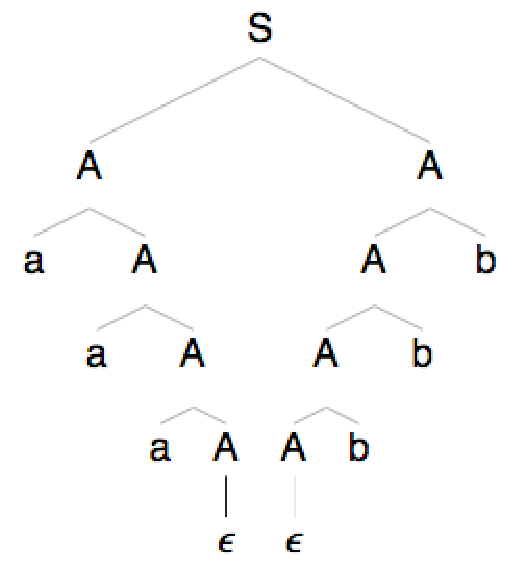
\includegraphics[scale=0.5]{figures/cfg1}
%\Tree [.S [.A a [.A a [.A a [.A $\epsilon$ ] ] ] ] [.A [.A [.A [.A $\epsilon$ ] b ] b ] b ] ]
\end{itemize}

\end{frame}

\begin{frame}
\frametitle{Context-Free Grammars}
\begin{itemize}
\item We will come back to this issue when we try to figure out whether human languages are more powerful than CFLs. 
\item The distinction between strings and the trees (or any kind of structural description) is called {\em weak} vs. {\em strong} generative capacity.
\end{itemize}

\end{frame}

\begin{frame}
\frametitle{Parse Trees}
\par\noindent
Consider the grammar with rules: 
\begin{eqnarray}
S &\rightarrow& \textit{NP}\ \textit{VP} \nonumber \\
\textit{NP} &\rightarrow& \textit{PRP} \nonumber \\
\textit{NP} &\rightarrow& \textit{DT}\ \textit{NPB} \nonumber \\
\textit{VP} &\rightarrow& \textit{VBP}\ \textit{NP} \nonumber \\
\textit{NPB} &\rightarrow& \textit{NN}\ \textit{NN} \nonumber \\
\textit{PRP} &\rightarrow& \textit{I} \nonumber \\
\textit{VBP} &\rightarrow& \textit{prefer} \nonumber \\
\textit{DT} &\rightarrow& \textit{a} \nonumber \\
\textit{NN} &\rightarrow& \textit{morning} \nonumber \\
\textit{NN} &\rightarrow& \textit{flight} \nonumber
\end{eqnarray}

\end{frame}

\begin{frame}
\frametitle{Parse Trees}

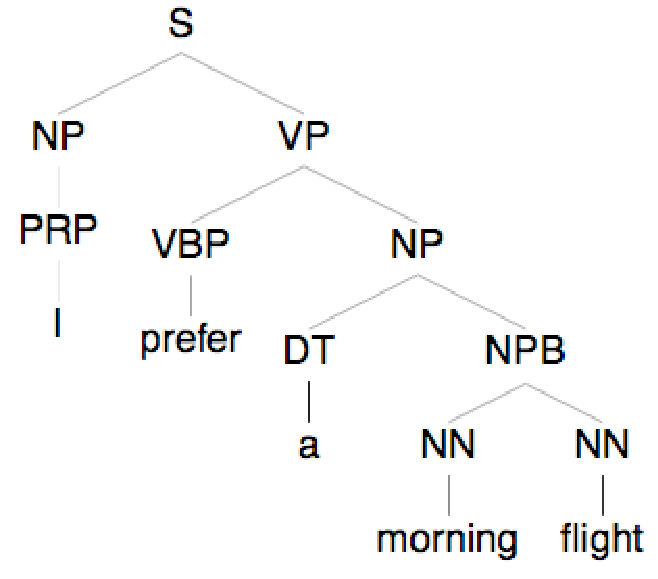
\includegraphics[scale=.5]{figures/cfg2}
%\Tree [.S [.NP [.PRP I ] ] [.VP [.VBP prefer ] [.NP [.DT a ] [.NPB [.NN morning ] [.NN flight ] ] ] ] ]

\end{frame}

\begin{frame}
\frametitle{Parse Trees: Equivalent Representations}
\begin{itemize}
\item (S (NP (PRP I) ) (VP (VBP prefer) (NP (DT a) (NPB (NN morning) (NN flight)))))
\item $[_{S}$ $[_{NP}$ $[_{PRP}$ I ] ] $[_{VP}$ $[_{VBP}$ prefer ]
$[_{NP}$ $[_{DT}$ a ] $[_{NPB}$ $[_{NN}$ morning ] $[_{NN}$ flight ] ] ] ] ]
\end{itemize}

\end{frame}

\begin{frame}
\frametitle{Ambiguous Grammars}
\begin{itemize}
\item $S \rightarrow S\ S$
\item $S \rightarrow a$
\item Given the above rules, consider the input {\em aaa}, what are the valid parse trees?
\item Now consider the input {\em aaaa}
\end{itemize}

\end{frame}

\end{document}
